\documentclass[tikz, border = 5pt]{standalone}

\begin{document}
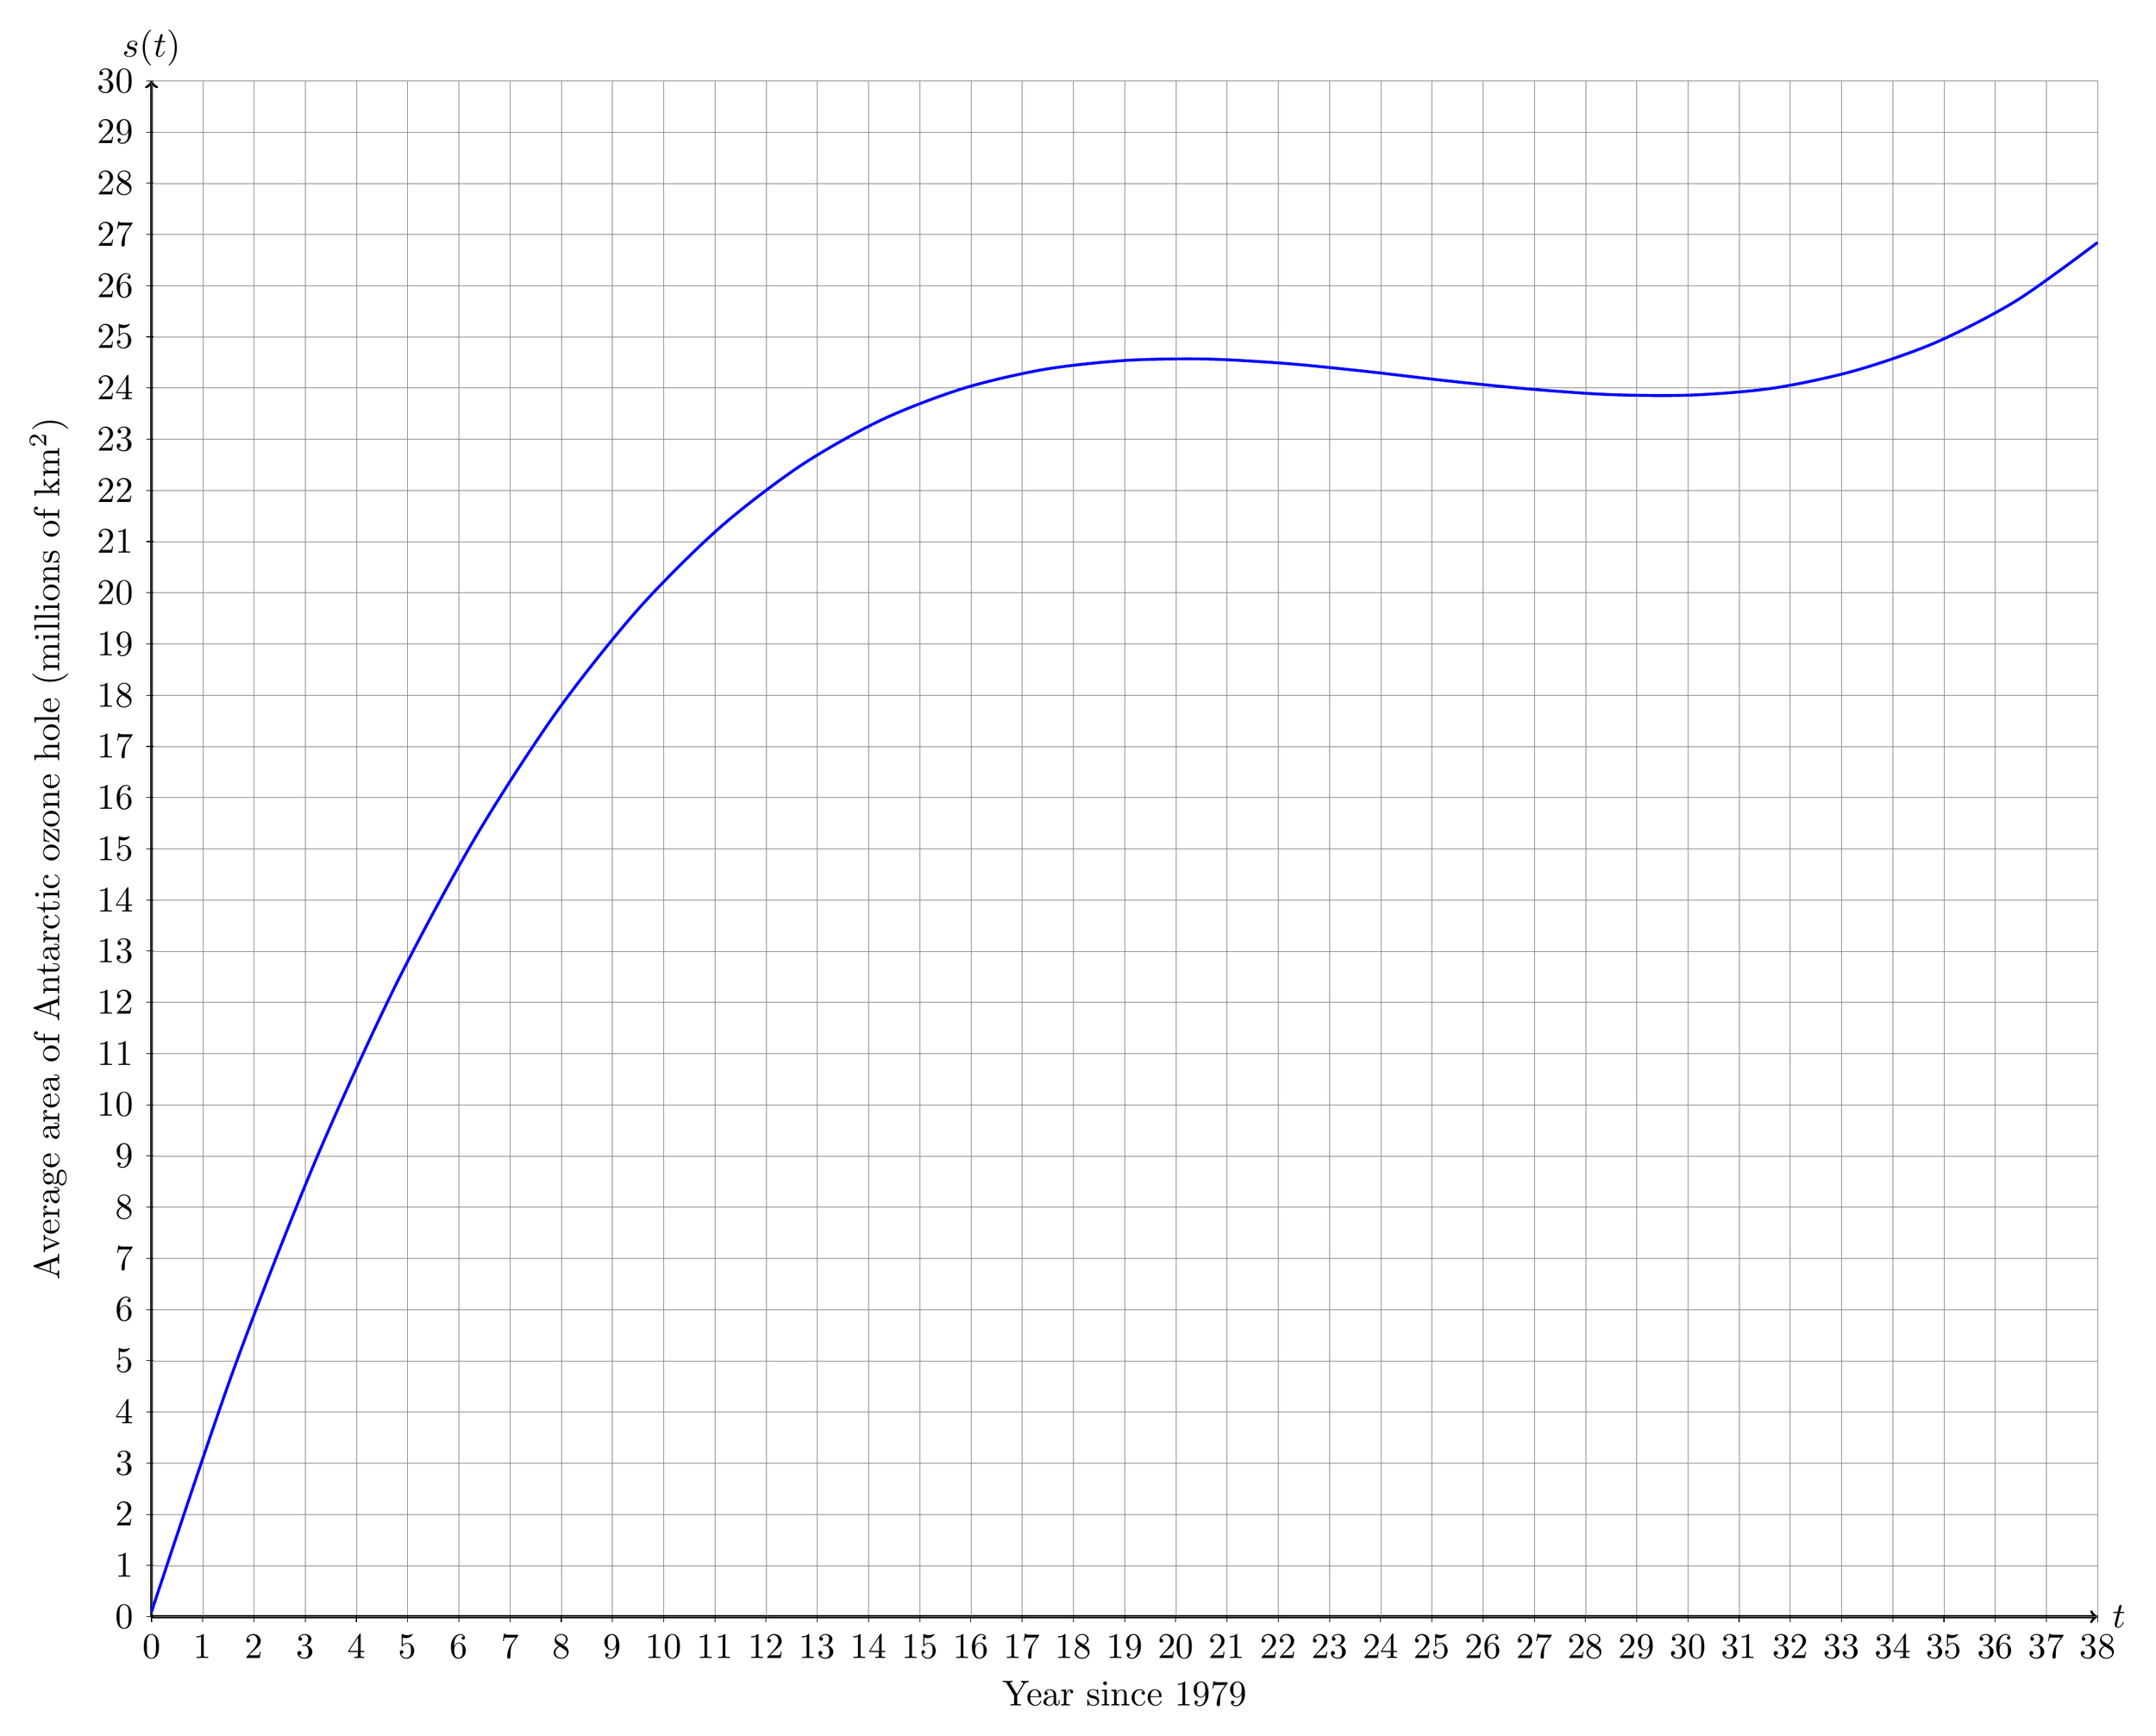
\begin{tikzpicture}
% axis
\draw[ultra thick, ->] (0, 0) -- (0, 30) node[above, black, scale=2] {$s(t)$};
\draw[ultra thick, ->] (0, 0) -- (38, 0) node[right, black, scale=2] {$t$};
\node[rotate=90, scale=2] at (-2,15) {Average area of Antarctic ozone hole (millions of km$^2$)};
\node[scale=2] at (19,-1.5) {Year since 1979};

% grid
\draw[help lines, step = 1cm] (0, 0) grid (38, 30);

%ticks
\foreach \x in {0,...,38}
  \draw (\x,1pt) -- (\x,-3pt) node[anchor=north, scale=2] {\x};
\foreach \y in {0,...,30}
  \draw (1pt,\y) -- (-3pt,\y) node[anchor=east, scale=2] {\y};

% graph
\draw[ultra thick, scale=1, domain=0:38,smooth,variable=\x, blue] plot ({\x},{0.001787*\x*\x*\x-0.1324*\x*\x+3.1576*\x+0.1});

\end{tikzpicture}
\end{document}
